\begin{frame}{IoT}

\centering
\Large{IoT with python and Raspberry Pi}\\
\textbf{PyDelhi 2016}
	
\end{frame}

\begin{frame}{Instructor}
	\begin{figure}
		\centering
		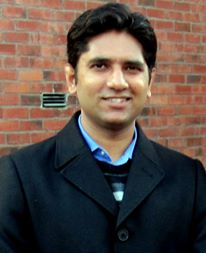
\includegraphics[width=4cm,height=4cm,keepaspectratio]{me}
	\end{figure}
	
	\centering
	\textcolor{blue}{Dr. Sandeep Nagar} \\
	M.Sc. Physics (MSU, Vadodara) \& PhD in Material Science \\ (Department of Material Science and Engineering, KTH, Sweden) \\
	contact e-mail: \textcolor{red}{sandeep.nagar@gmail.com}
\end{frame}

\begin{frame}{Why would I do IoT?}
	\begin{itemize}
		\item Its for everybody!
		\item Started just for fun
		\item Some serious experimentation
		\item Making scientific instruments
		\item Internet control gives multi-functionality to experiments
	\end{itemize}
\end{frame}

\begin{frame}{Outline of workshop}
	\begin{enumerate}
		\item Introduction to IoT and Raspberry Pi ($30$ Minutes)
		\begin{itemize}
			\item Intro to IoT
			\item Various parts
			\item Installing OS
		\end{itemize}
		\item Accessing GPIO pins ($30$ minutes)
		\begin{itemize}
			\item Writing to GPIO pins
			\item Reading from GPIO pins
		\end{itemize}
		\item IoT with RPi ($30$ minutes)
		\begin{itemize}
			\item Running RPi headless 
			\item Adding sensors
			\item Interacting with data generated using IoT device
		\end{itemize}
	\end{enumerate}
\end{frame}

\section{Intro to IoT}

\begin{frame}{Introduction to IoT}
	\begin{itemize}
		\item IoT is a connecting \textbf{things} to internet
		\item Two types:
		\begin{itemize}
			\item Device computes locally and interacts on internet
			\item Device does not compute locally but interacts on internet
		\end{itemize}
		\item Interaction on internet means:
		\begin{itemize}
			\item Write and read data
			\item Write and read code to control systems
		\end{itemize}
	\end{itemize}
\end{frame}

\begin{frame}{Intro to RPi}
	\begin{itemize}
		\item Microcomputer
		\begin{itemize}
			\item Credit card sized ($20 \times 10$ cm)
			\item Weight = $68$ g
		\end{itemize}
		\item Very cost effective
		\begin{itemize}
			\item Presently available for INR $2,875$ at amazon 
		\end{itemize}
		\item Low power consumption 
		\begin{itemize}
			\item We will use mobile phone charger
		\end{itemize}
		\item Remote access over internet
		\begin{itemize}
			\item We will use a LAN cable for connectivity
		\end{itemize}
		\item Runs Linux
		\begin{itemize}
			\item Raspbian is a version of Debian optimized for RPi
		\end{itemize}
	\end{itemize}
\end{frame}

\begin{frame}{Powerful IoT platform}
	\begin{itemize}
		\item Broadcom $900$ MHz BCM$2836$ ARMv$7$ Quad Core Processor SoC 
		\item Broadcom VideoCore IV GPU
		\item $1$ GB RAM
		\item Expanded $40$-pin GPIO Header
		\item $4$ x USB$2.0$ Ports with up to $1.2$A output
		\item $4$ pole Stereo output and Composite video port
		\item Full size HDMI
		\item CSI camera port for connecting the Raspberry Pi camera
		\item DSI display port for connecting the Raspberry Pi touch screen display
		\item Micro SD port for loading your operating system and storing data
		\item Micro USB power source
	\end{itemize}
	Ref: \url{https://www.raspberrypi.org/products/raspberry-pi-2-model-b/}
\end{frame}

\begin{frame}{RPi}
	\begin{figure}
		\centering
		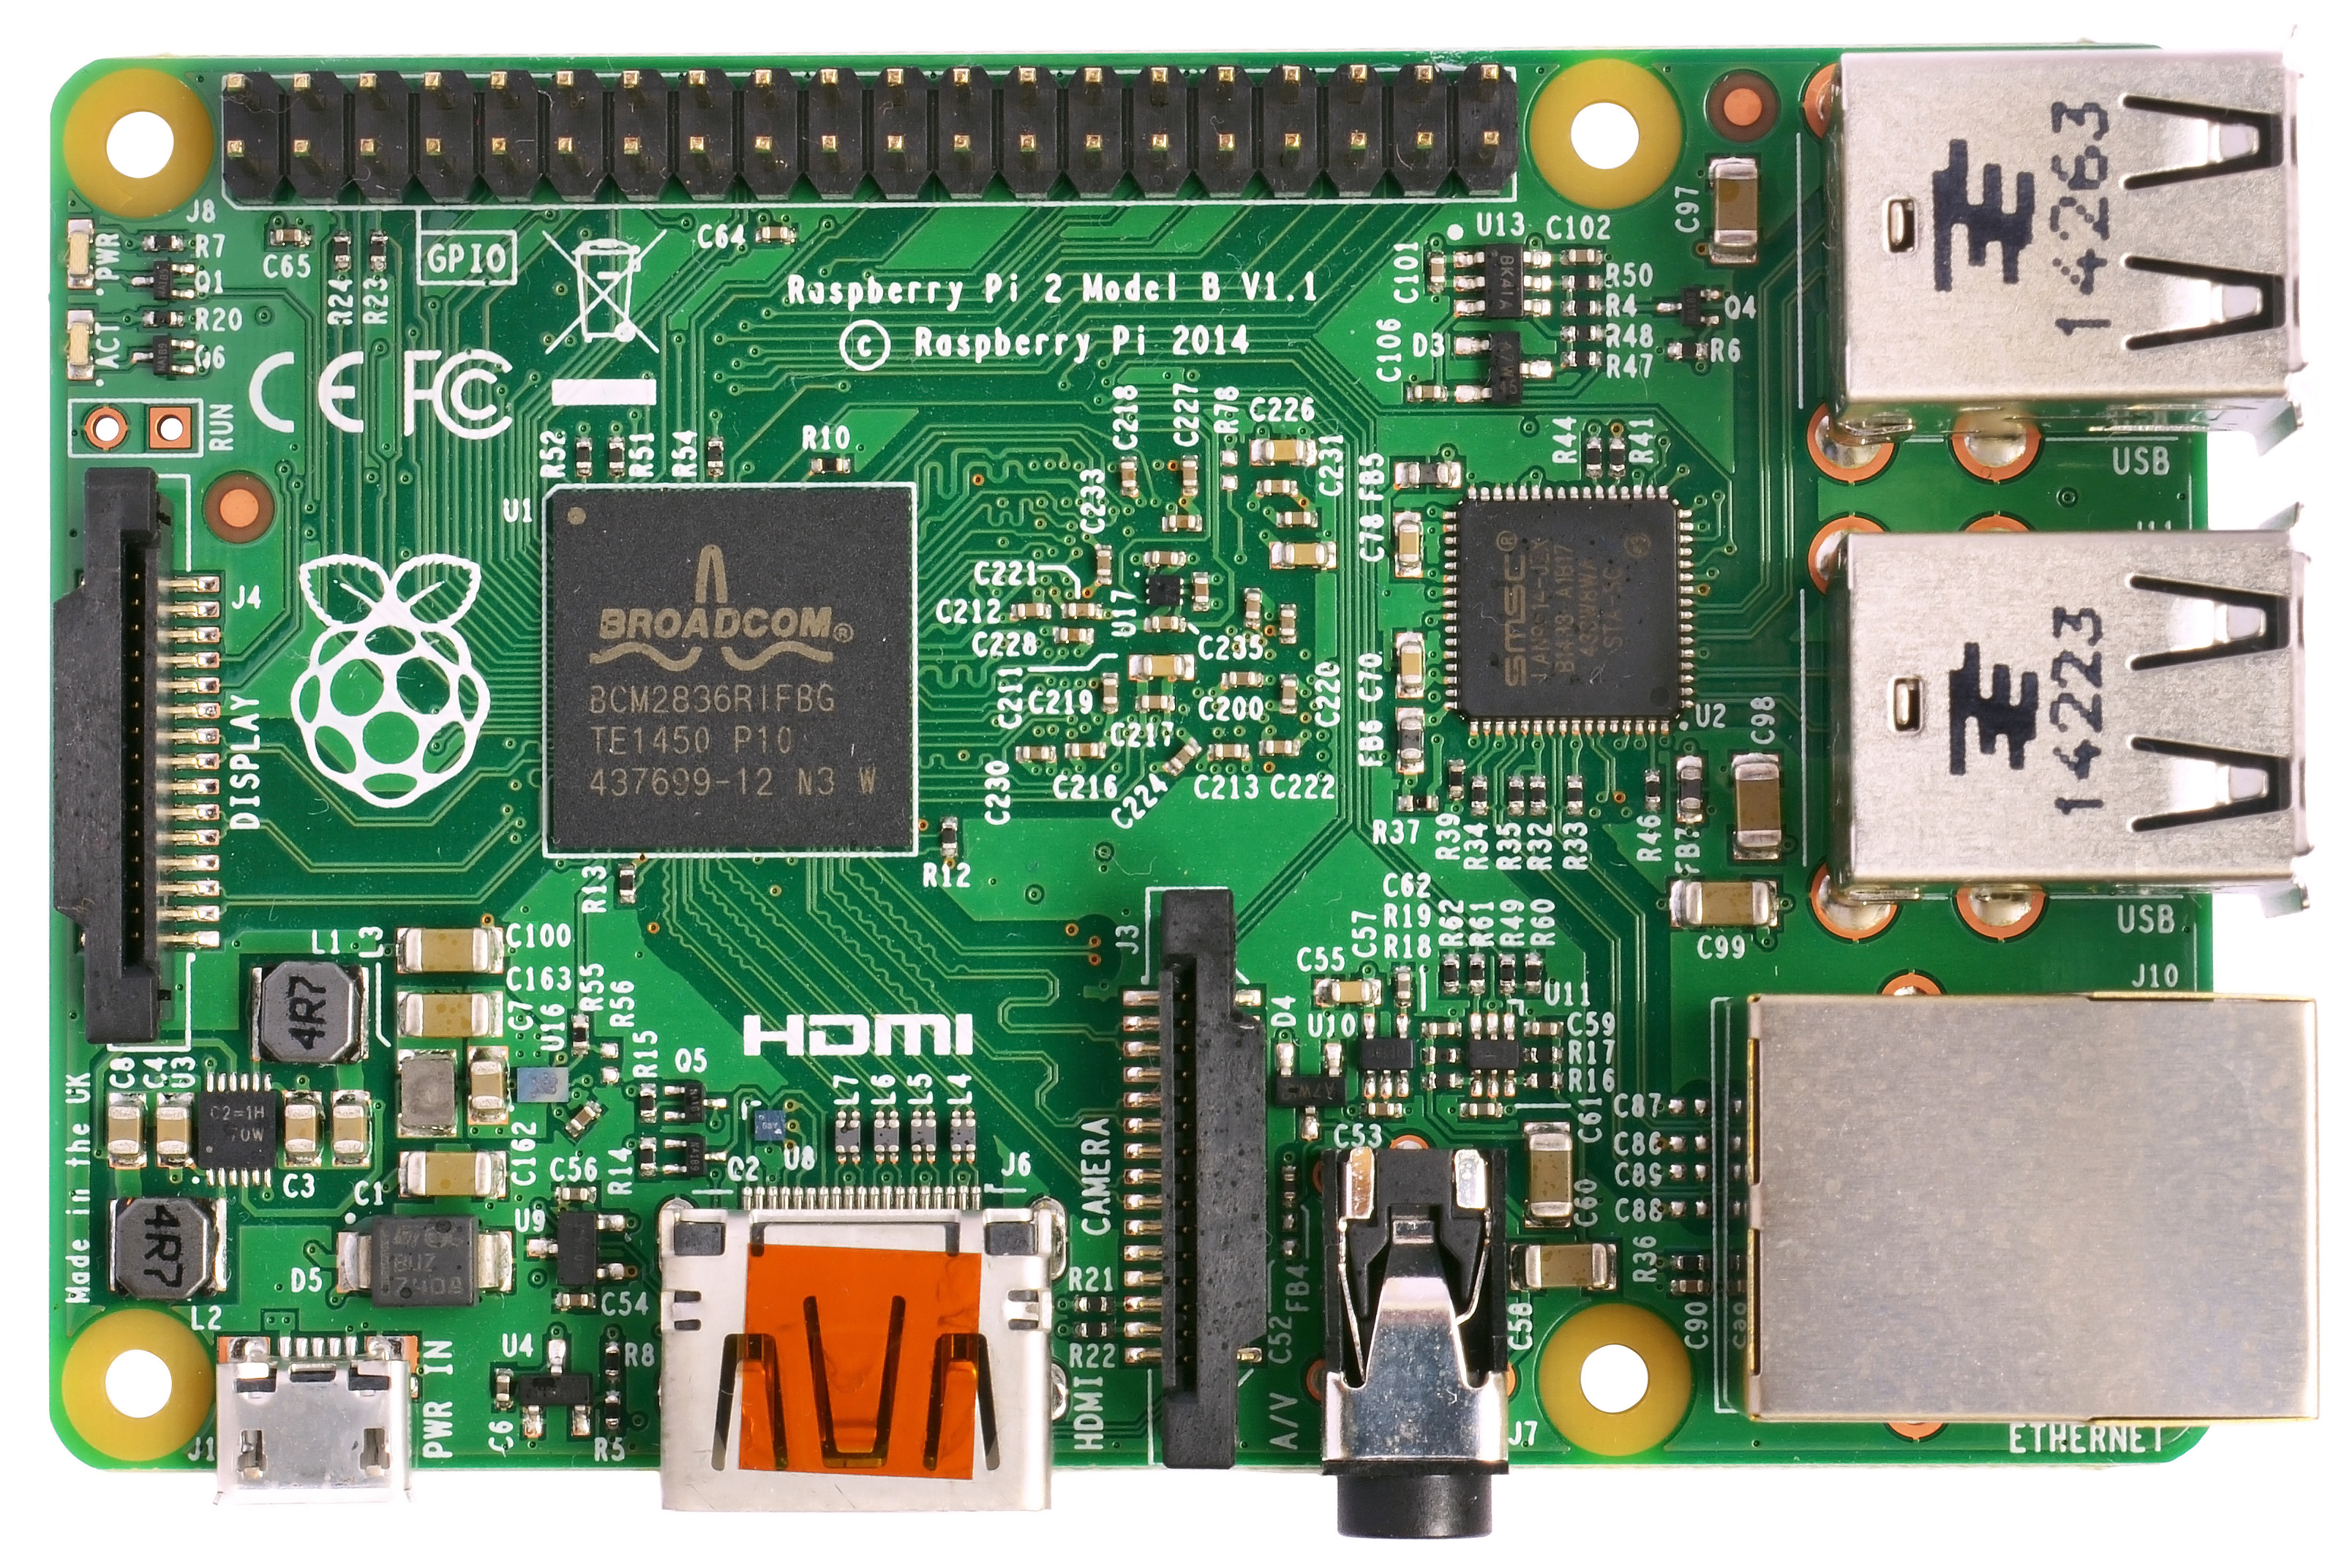
\includegraphics[width=10cm,height=10cm,keepaspectratio]{RPi2}
		\caption{Top portion of Raspberry Pi 2 Model B}
	\end{figure}
\end{frame}

\begin{frame}{OS}
	\begin{itemize}
		\item OS is installed on a micro SD card
		\item Raspbian is optimized OS for RPi
		\item Available at \url{https://www.raspbian.org/}
		\item Micro SD cards with pre-installed OS are also available
		\item Installation
		\begin{itemize}
			\item Format the card
			\item Install NOOBS
			\item Choose Raspbian
			\item Install
		\end{itemize} 
	\end{itemize}
\end{frame}